%%novalidate
\newpage
\section{Destination Tickets \& Effective Resistance}

\subsection{Destination Tickets \& Winning}
An obvious strategy in \textit{Ticket to Ride} is to collect
Destination Tickets and buy routes so as to connect them.
We investigate the effect of collecting Destination Tickets
on winning the game.
We simulate 10,000 two-player and 10,000 four-player games
using Silva et al.'s program.
For each Destination Ticket, we calculate the proportion of 
games that the player holding the Destination Ticket won.
For example, players in two-player games with Phoenix to Portland
won almost exactly half of their games.
Our results appear in \cref{fig:tickets}.

\end{multicols}
\begin{figure}[h]
\centering
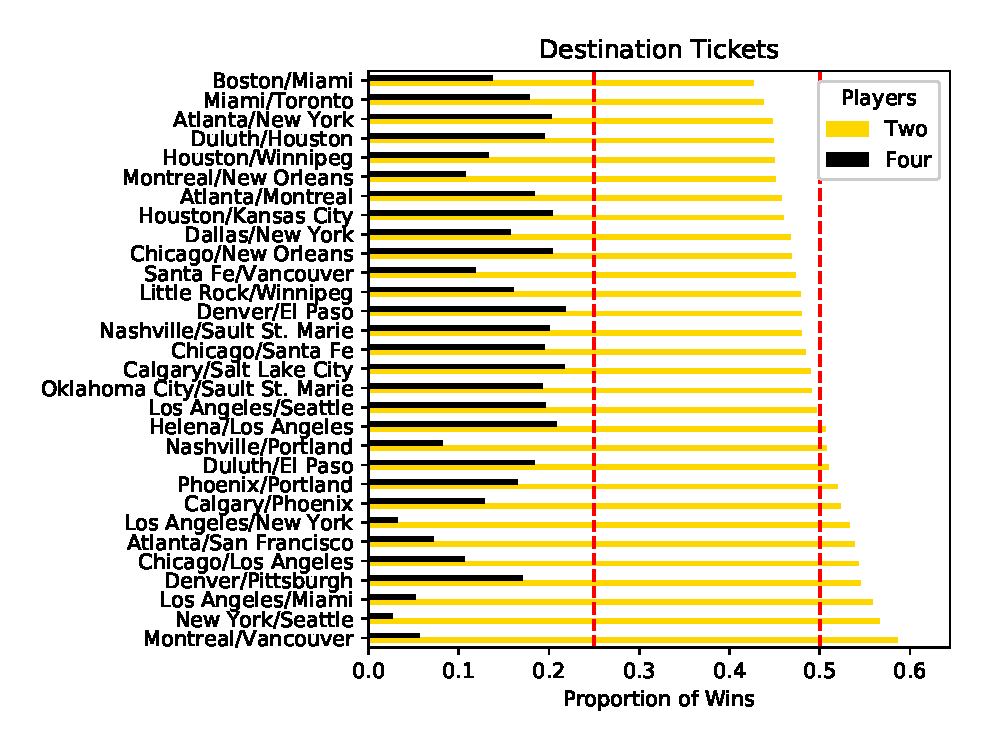
\includegraphics[scale=.8]{figures/destination_tickets}
\caption{For each Destination Ticket,
the proportion of two-player and four-player games that 
the player with the Destination Ticket won.
The vertical red lines at $1/4$ and $1/2$ represent
the expected proportion of games players would win
if Destination Tickets had no effect.}
\label{fig:tickets}
\end{figure}
\begin{multicols}{2}

The vertical red lines at $1/4$ and $1/2$ indicate
the expected proportion of wins if Destination Tickets
had no effect on winning: players in two-player games
would win half the time and players in four-player games
would win a quarter of the time.

Remarkably, there are no Destination Tickets in four-player
games that win more than $25\%$ of all games.
This would be impossible if all players had the same number
of Destination Tickets because \textit{some} player must win every
game.
Therefore the implication is that players who spend their
turns collecting more Destination Tickets win less frequently
than those who take Train Cards or claim routes.
Within the set of Destination Tickets in four-player games,
some still do even worse.
New York to Seattle, Los Angeles to New York, Los Angeles to Miami,
and Montreal to Vancouver have especially low win rates.
A quick inspection of \cref{fig:board} shows that all four pairs of cities
are particularly far apart (in terms of both geography and the
length of the shortest paths between them).
Perhaps these longer Destination Tickets are harder to connect and,
in the common case that players cannot connect them, subtract an insurmountable
number of points from players' final scores.

Destination Tickets in two-player games also mostly fall
below the threshold of wins we would expect if there were
no relationship between winning and Destination Tickets.
But, unlike four-player games, some Destination Tickets
win more than expected: Montreal to Vancouver,
Los Angeles to Miami, Chicago to Los Angeles, and
Denver to Pittsburgh.
Ironically, the cities that won the least often in four-player
games now win the most often in two-player games.
Perhaps the longer Destination Tickets are easier
to connect in two-player than four-player games
and, unlike the other Destination Tickets, add
a substantial number of points to the final score.

We dive into the math to explore the deeper structure
of Destination Tickets.

\subsection{Effective Resistance}

Can effective resistance help?
\begin{figure*}[!ht]
\centering
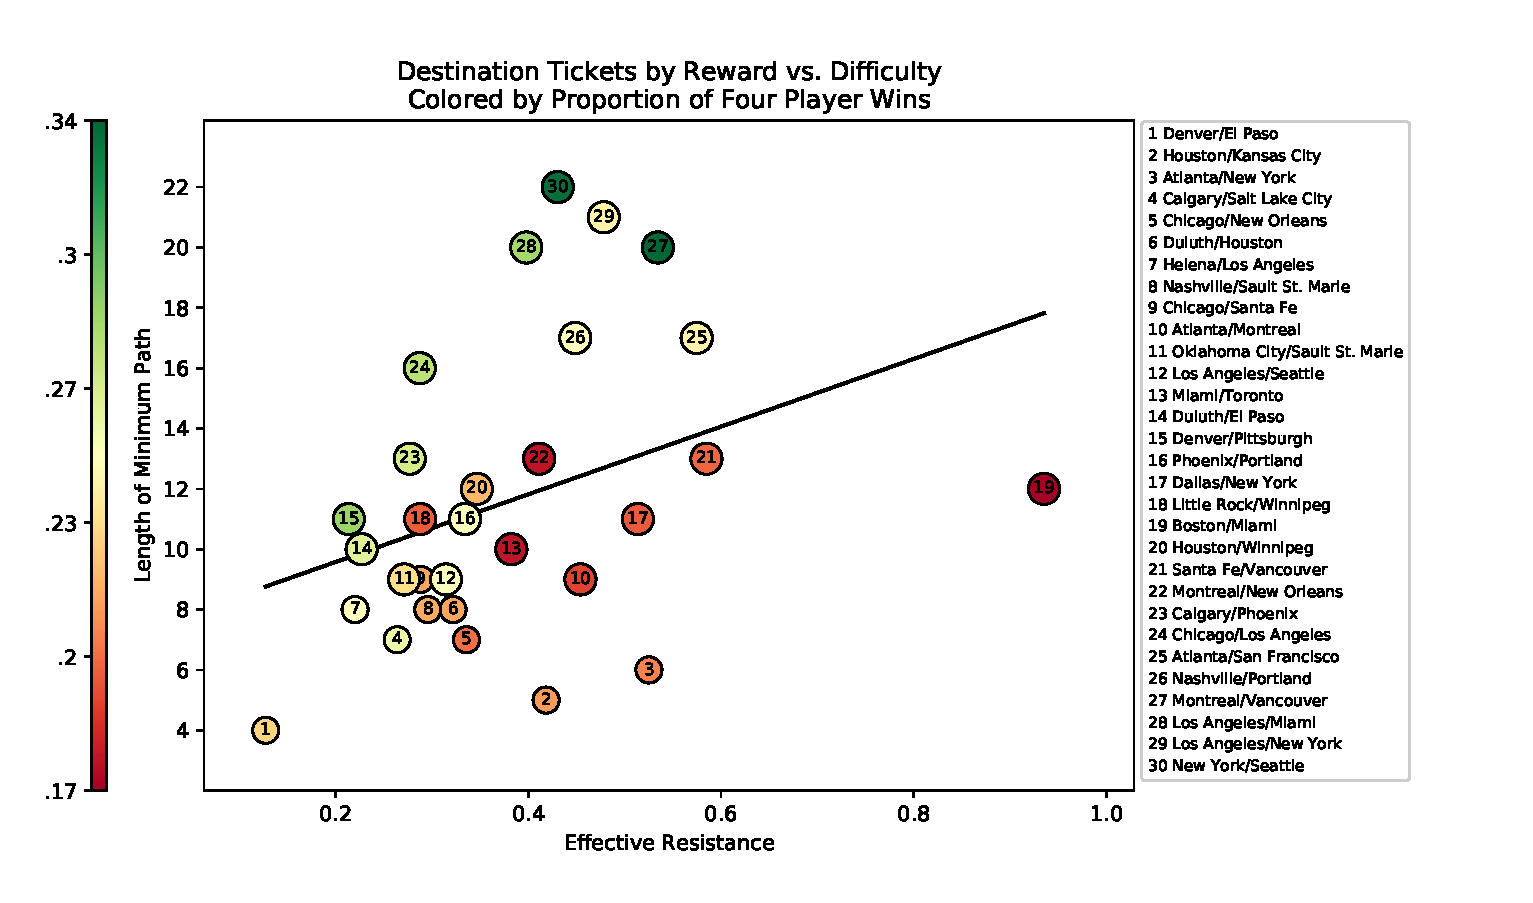
\includegraphics[scale=.8]{figures/resistance_four}
\caption{Destination Tickets by their effective
resistance and minimum path length.
The line of best fit gives an approximation of the
Destination Tickets that are better deals (above the line).
Note: the $16^{th}$ Destination Ticket Portland/Phoenix is obscured
by the $18^{th}$.}
\label{fig:resistance}
\end{figure*}

\begin{figure*}[!h]
\centering
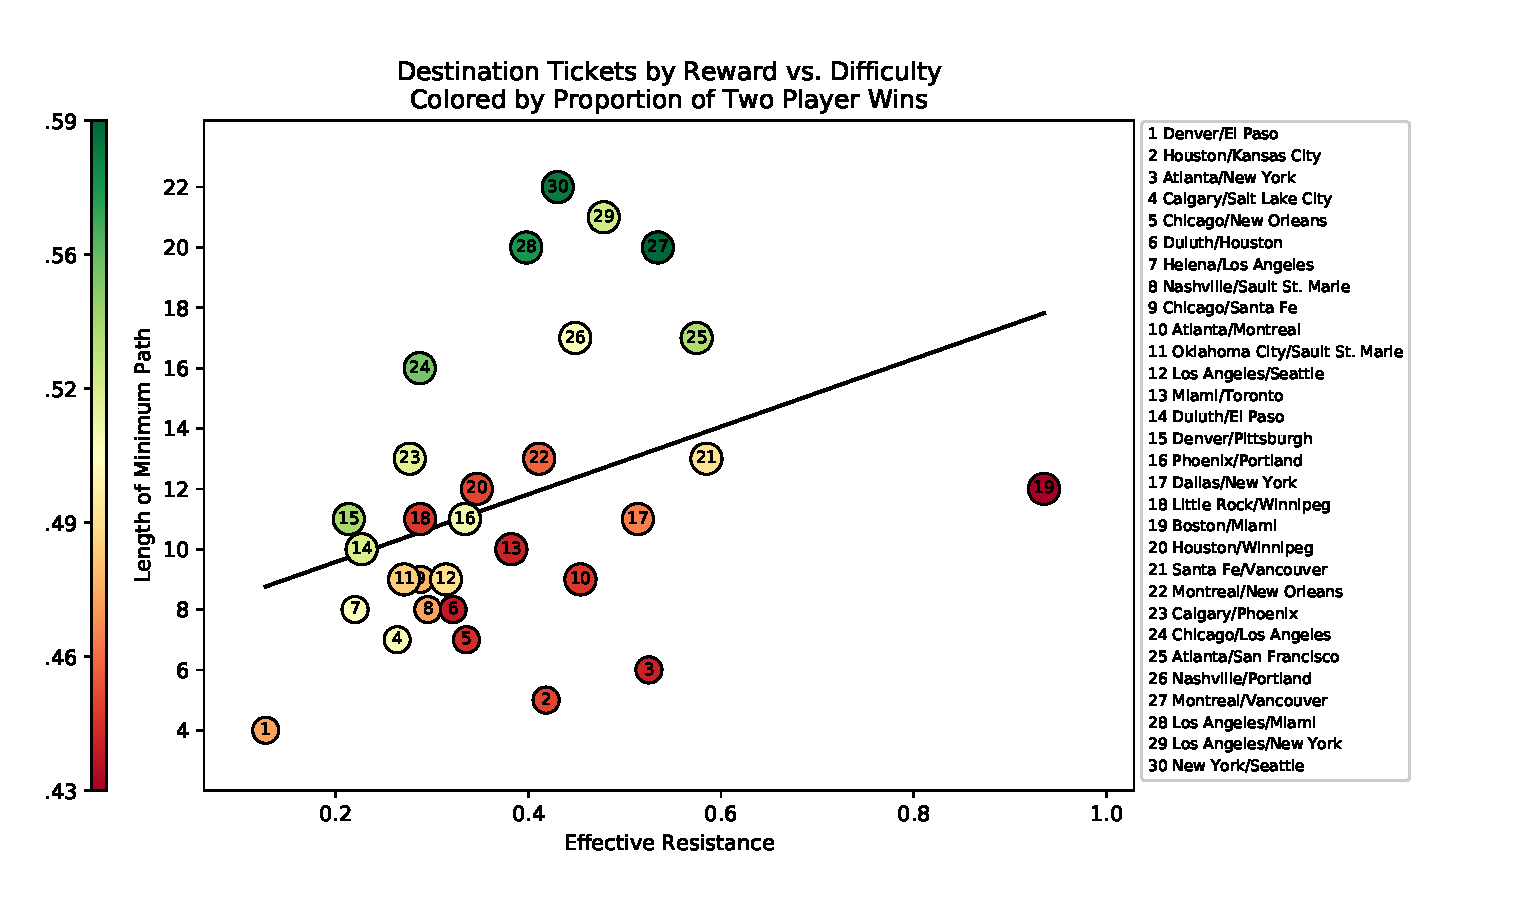
\includegraphics[scale=.8]{figures/resistance_two}
\caption{Destination Tickets by their effective
resistance and minimum path length.
The line of best fit gives an approximation of the
Destination Tickets that are better deals (above the line).
Note: the $16^{th}$ Destination Ticket Portland/Phoenix is obscured
by the $18^{th}$.}
\label{fig:resistance}
\end{figure*}
